\documentclass[10pt]{exam}
\usepackage[hon]{template-for-exam}
\usepackage{pgfplots,multicol}
\pgfplotsset{
    compat=1.18,
    reg/.append style={
        xmin =-4.5,
        xmax =4.5,
        ymin =-4.5,
        ymax = 4.5,
        axis lines = center,
        xtick = {-4,...,4},
        ytick = {-4,...,4},
        height = 6cm,
        width = 6cm,
        grid = major,
        grid style = {thick, dotted},
        tick label style = {font=\small}
      },
    pulseplot/.append style={
      xmin =-6.5,
      xmax = 6.5,
      ymin =-2.5,
      ymax = 2.5,
      axis lines = center,
      xtick = {-6,...,6},
      ytick = {-2,...,2},
      height = 5cm,
      width = 7.5cm,
      grid = major,
      grid style = {thick, dotted},
      tick label style = {font=\small}
    },
    myplot/.append style={
      smooth,domain=-6:6,samples=50,thick
    },
  }
\pgfmathdeclarefunction{gauss}{2}{%
  \pgfmathparse{1/(#2*sqrt(2*pi))*exp(-((x-#1)^2)/(2*#2^2))}%
}

\title{Waves}
\author{Rohrbach}
\date{\today}

\begin{document}
\maketitle


\subsection*{Superposition}

\vfill


  \begin{tikzpicture}
    \def\plotsep{4}

    \draw (6.5,3)  -- ++(0,-15);

    \begin{scope}
      \begin{scope}
        \node[anchor=east] at (0,1.8) {$t=\SI{0}{\second}$};
        \begin{axis}[pulseplot]
          \addplot[myplot, ultra thick] {1.3*(gauss(-4,.5)+gauss(4,.5))};
        \end{axis}
      \end{scope}
      
      \begin{scope}[shift={(0,-\plotsep)}]
        \node[anchor=east] at (0,1.8) {$t=\SI{1}{\second}$};
        \begin{axis}[pulseplot]
          \addplot[myplot, ultra thick] {1.3*(gauss(-2,.5)+gauss(2,.5))};
        \end{axis}
      \end{scope}
  
      \begin{scope}[shift={(0,-2*\plotsep)}]
        \node[anchor=east] at (0,1.8) {$t=\SI{2}{\second}$};
        \begin{axis}[pulseplot]
        \end{axis}
      \end{scope}


      \begin{scope}[shift={(0,-3*\plotsep)}]
        \node[anchor=east] at (0,1.8) {$t=\SI{3}{\second}$};
        \begin{axis}[pulseplot]
        \end{axis}
      \end{scope}
  
    \end{scope}

    \begin{scope}[shift={(8,0)}]
      \begin{scope}
        \node[anchor=east] at (0,1.8) {$t=\SI{0}{\second}$};
        \begin{axis}[pulseplot]
          \addplot[myplot, ultra thick] {1.3*(gauss(-4,.5)-gauss(4,.5))};
        \end{axis}
      \end{scope}
      
      \begin{scope}[shift={(0,-\plotsep)}]
        \node[anchor=east] at (0,1.8) {$t=\SI{1}{\second}$};
        \begin{axis}[pulseplot]
          \addplot[myplot, ultra thick] {1.3*(gauss(-2,.5)-gauss(2,.5))};
        \end{axis}
      \end{scope}
  
      \begin{scope}[shift={(0,-2*\plotsep)}]
        \node[anchor=east] at (0,1.8) {$t=\SI{2}{\second}$};
        \begin{axis}[pulseplot]
        \end{axis}
      \end{scope}


      \begin{scope}[shift={(0,-3*\plotsep)}]
        \node[anchor=east] at (0,1.8) {$t=\SI{3}{\second}$};
        \begin{axis}[pulseplot]
        \end{axis}
      \end{scope}
  
    \end{scope}
  \end{tikzpicture}


\subsection*{Interference}



\begin{center}
  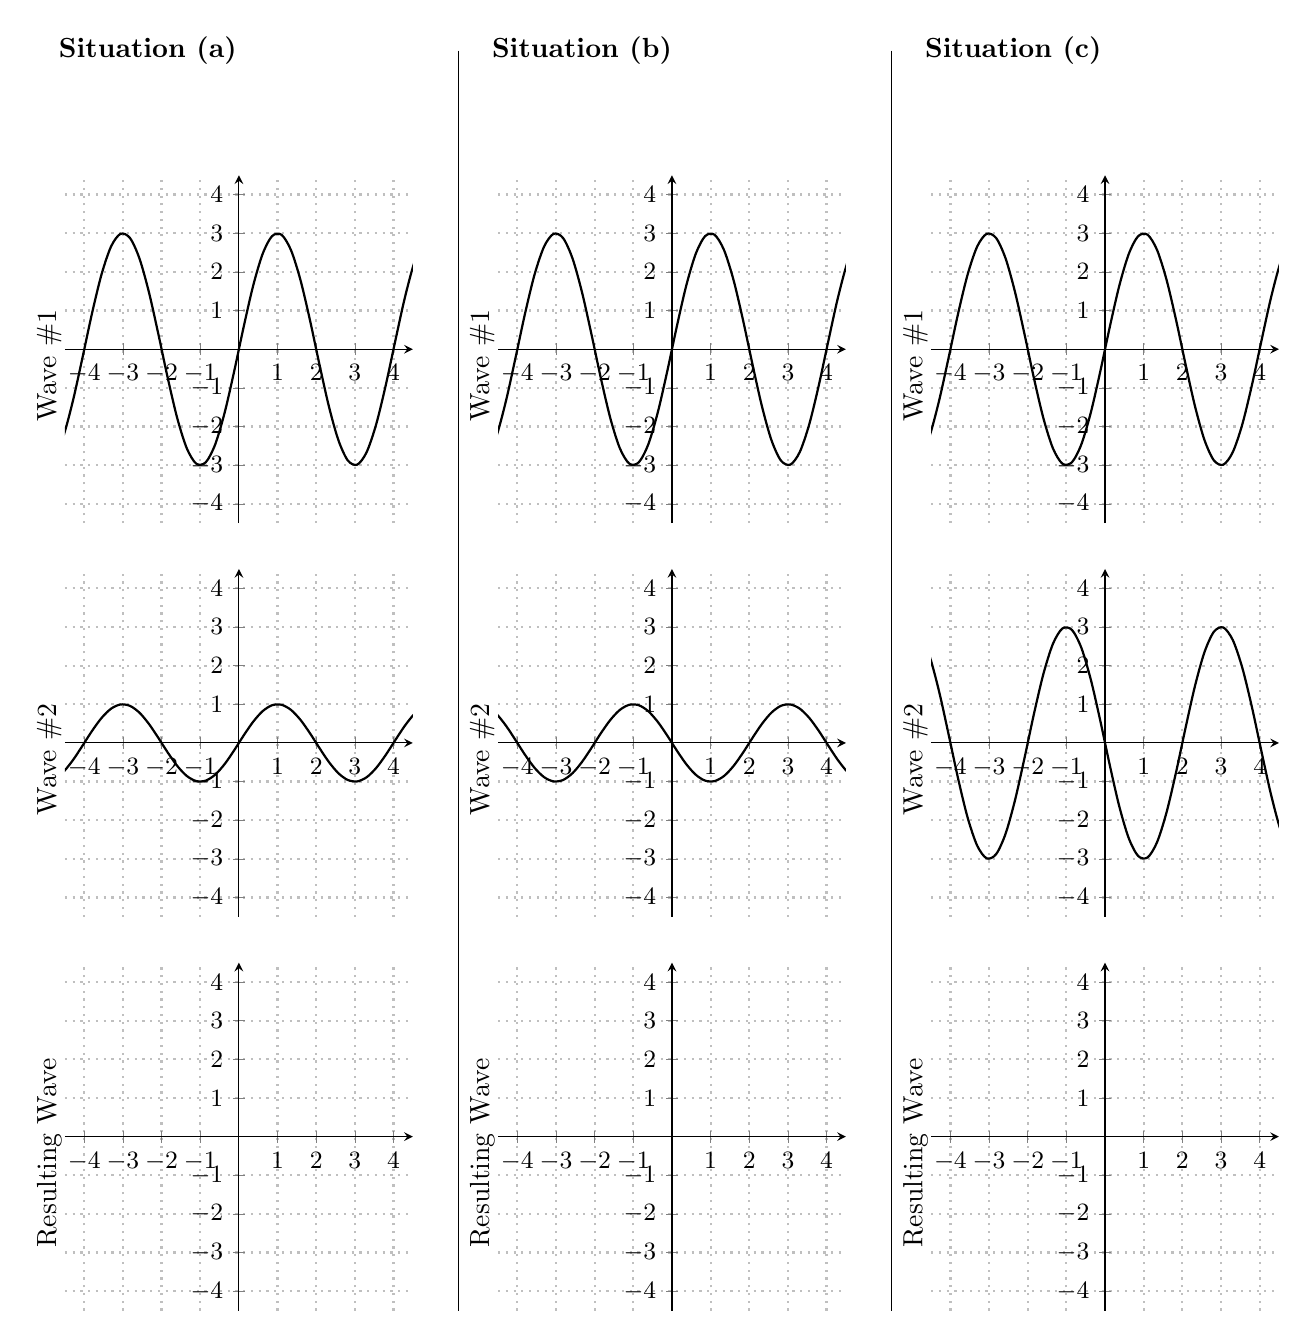
\begin{tikzpicture}
    \draw (5,6)  -- ++(0,-16);
    \draw (10.5,6)  -- ++(0,-16);
  
    \begin{scope}
      \node[anchor=west] at (-.2,6) {\bf Situation (a)};
      \begin{scope}
          \node[rotate=90] at (-.2,2) {Wave \#1};
          \begin{axis}[reg]
            \addplot[myplot] {3*sin(deg(2*pi*x/4))};
          \end{axis}
      \end{scope}
      
      \begin{scope}[shift={(0,-5)}]
        \node[rotate=90] at (-.2,2) {Wave \#2};
        \begin{axis}[reg]
          \addplot[myplot] {1*sin(deg(2*pi*x/4))};
        \end{axis}
      \end{scope}
  
      \begin{scope}[shift={(0,-10)}]
        \node[rotate=90] at (-.2,2) {Resulting Wave};
        \begin{axis}[reg]
        \end{axis}
      \end{scope}
  
    \end{scope}
      
    \begin{scope}[shift={(5.5,0)}]
  
      \node[anchor=west] at (-.2,6) {\bf Situation (b)};
      \begin{scope}
        \node[rotate=90] at (-.2,2) {Wave \#1};
          \begin{axis}[reg]
            \addplot[myplot] {3*sin(deg(2*pi*x/4))};
          \end{axis}
      \end{scope}
      
      \begin{scope}[shift={(0,-5)}]
        \node[rotate=90] at (-.2,2) {Wave \#2};
        \begin{axis}[reg]
          \addplot[myplot] {-1*sin(deg(2*pi*x/4))};
        \end{axis}
      \end{scope}
  
      \begin{scope}[shift={(0,-10)}]
        \node[rotate=90] at (-.2,2) {Resulting Wave};
        \begin{axis}[reg]
        \end{axis}
      \end{scope}
  
    \end{scope}
  
    \begin{scope}[shift={(11,0)}]
  
      \node[anchor=west] at (-.2,6) {\bf Situation (c)};
      \begin{scope}
        \node[rotate=90] at (-.2,2) {Wave \#1};
          \begin{axis}[reg]
            \addplot[myplot] {3*sin(deg(2*pi*x/4))};
          \end{axis}
      \end{scope}
      
      \begin{scope}[shift={(0,-5)}]
        \node[rotate=90] at (-.2,2) {Wave \#2};
        \begin{axis}[reg]
          \addplot[myplot] {-3*sin(deg(2*pi*x/4))};
        \end{axis}
      \end{scope}
  
      \begin{scope}[shift={(0,-10)}]
        \node[rotate=90] at (-.2,2) {Resulting Wave};
        \begin{axis}[reg]
        \end{axis}
      \end{scope}
  
    \end{scope}
  
  \end{tikzpicture}
\end{center}





\subsection*{Resonance}


\vfill

\subsection*{Standing Waves}
  
  
  
\subsection*{Beats}
  

  
    \begin{tikzpicture}
      \node at (0,0) 
        {\includegraphics[width=12cm]{Fig20_21.jpg}};
      \fill[white] (-3,-1) rectangle (6,.26);
    \end{tikzpicture}
  
    Take a look at the illustration below that refers to a wave of frequency 10 Hz being played at the same time as a wave of frequency 12 Hz.
  
  \centering\includegraphics[width=6cm]{Figure.png}
  
  
    Draw your own beats!  Draw two bugs jumping on the water.  One bug jumps forward 3 cm each hop; the other bug jumps forward 4 cm each hop.
  
    \begin{tikzpicture}
      \draw[dotted] (0,0) grid[step=0.5] (15,-1.5);
    \end{tikzpicture}


  \begin{multicols}{3}
    \footnotesize
    \centering

    \begin{tabular}{ccc}
      Concert & B$\flat$ Trumpet & Frequency \\
      Pitch   &  Pitch & (Hz) \\
      \hline\hline
      A$\sharp$3 & C4 & 233.08 \\
      B3 & C$\sharp$4 & 246.94 \\
      C4 & D4 & 261.63 \\
      C$\sharp$4 & D$\sharp$4 & 277.18 \\
      D4 & E4 & 293.66 \\
      D$\sharp$4 & F4 & 311.13 \\
      E4 & F$\sharp$4 & 329.63 \\
      F4 & G4 & 349.23 \\
      F$\sharp$4 & G$\sharp$4 & 369.99 \\
      G4 & A4 & 392.00 \\
      G$\sharp$4 & A$\sharp$4 & 415.30 \\
      A4 & B4 & 440.00 \\
      \hline
    \end{tabular}

    \begin{tabular}{ccc}
      Concert & B$\flat$ Trumpet & Frequency \\
      Pitch   &  Pitch & (Hz) \\
      \hline\hline
      A$\sharp$4 & C5 & 466.16 \\
      B4 & C$\sharp$5 & 493.88 \\
      C5 & D5 & 523.25 \\
      C$\sharp$5 & D$\sharp$5 & 554.37 \\
      D5 & E5 & 587.33 \\
      D$\sharp$5 & F5 & 622.25 \\
      E5 & F$\sharp$5 & 659.25 \\
      F5 & G5 & 698.46 \\
      F$\sharp$5 & G$\sharp$5 & 739.99 \\
      G5 & A5 & 783.99 \\
      G$\sharp$5 & A$\sharp$5 & 830.61 \\
      A5 & B5 & 880.00 \\
      \hline
    \end{tabular}

    \begin{tabular}{ccc}
      Concert & B$\flat$ Trumpet & Frequency \\
      Pitch   &  Pitch & (Hz) \\
      \hline\hline
      A$\sharp$5 & C6 & 932.33 \\
      B5 & C$\sharp$6 & 987.77 \\
      C6 & D6 & 1046.50 \\
      C$\sharp$6 & D$\sharp$6 & 1108.73 \\
      D6 & E6 & 1174.66 \\
      D$\sharp$6 & F6 & 1244.51 \\
      E6 & F$\sharp$6 & 1318.51 \\
      F6 & G6 & 1396.91 \\
      F$\sharp$6 & G$\sharp$6 & 1479.98 \\
      G6 & A6 & 1567.98 \\
      G$\sharp$6 & A$\sharp$6 & 1661.22 \\
      A6 & B6 & 1760.00 \\
      \hline
      A$\sharp$6 & C7 & 1864.66 \\
      \hline
    \end{tabular}
    
  \end{multicols}
  


\end{document}